\chapter{Principes fondamentaux de machine learning}
\label{chap:fondamentaux_ml}

\par{Ce chapitre va permettre d’avoir les bases nécessaires pour comprendre ce qu’est le machine learning, ses limites et ses applications.}

% --------------------------------------------------------------------------------------------

\section{Introduction au machine learning}

\par{L'apprentissage automatique (machine learning) est une branche de l'intelligence artificielle qui permet à un programme d'automatiser l'apprentissage à partir d'exemples, sans être explicitement programmé pour accomplir une tâche.}

\par{Les principaux algorithmes de machine learning peuvent se diviser en 2 catégories :
\begin{itemize}
    \item Apprentissage supervisé : le modèle est entraîné avec des données étiquetées et il doit apprendre à reconnaître les patrons pour prédire les résultats futurs. Quelques exemples :
    \begin{itemize}
        \item Réseaux de neurones : est comme une équipe de détectives qui examinent ensemble une image pour décider si elle représente un chien, un chat ou un arbre, en se basant sur les caractéristiques qu'ils ont appris à reconnaître.
        \item Régression linéaire : vise à prédire une valeur continue (par exemple, la température) en fonction de variables explicites.
        \item Les arbres de décision : un algorithme qui utilise des règles pour prendre des décisions en fonction de caractéristiques des données.
    \end{itemize}
    \item Apprentissage non supervisé : le modèle est entraîné avec des données non étiquetées et il doit apprendre à identifier les groupes ou les tendances dans les données. Quelques exemples :
    \begin{itemize}
        \item L'agrégation (cluster) : un algorithme qui vise à grouper les données en fonction de leurs similarités.
        \item Autoencodeurs : réseau de neurones qui permettent la compression (encodeur) et décompression (décodeur) de données
        \item Analyse en composantes principales (PCA) : permet de réduire une grande base de données de caractéristiques par exemple de vins (degré d'alcool, la couleur, l'acidité, etc.) à seulement deux ou trois caractéristiques les plus importantes qui expliquent le plus de variabilité dans les vins, pour faciliter leur comparaison et leur classification.
    \end{itemize}
\end{itemize}}

\par{La figure~\ref{fig:A1_01_resume_machine_learning_supervise} permet d'avoir un aperçu des phases de création d'un modèle de machine learning à partir d'un algorithme supervisé.}

\begin{figure}[H]
    \centering
    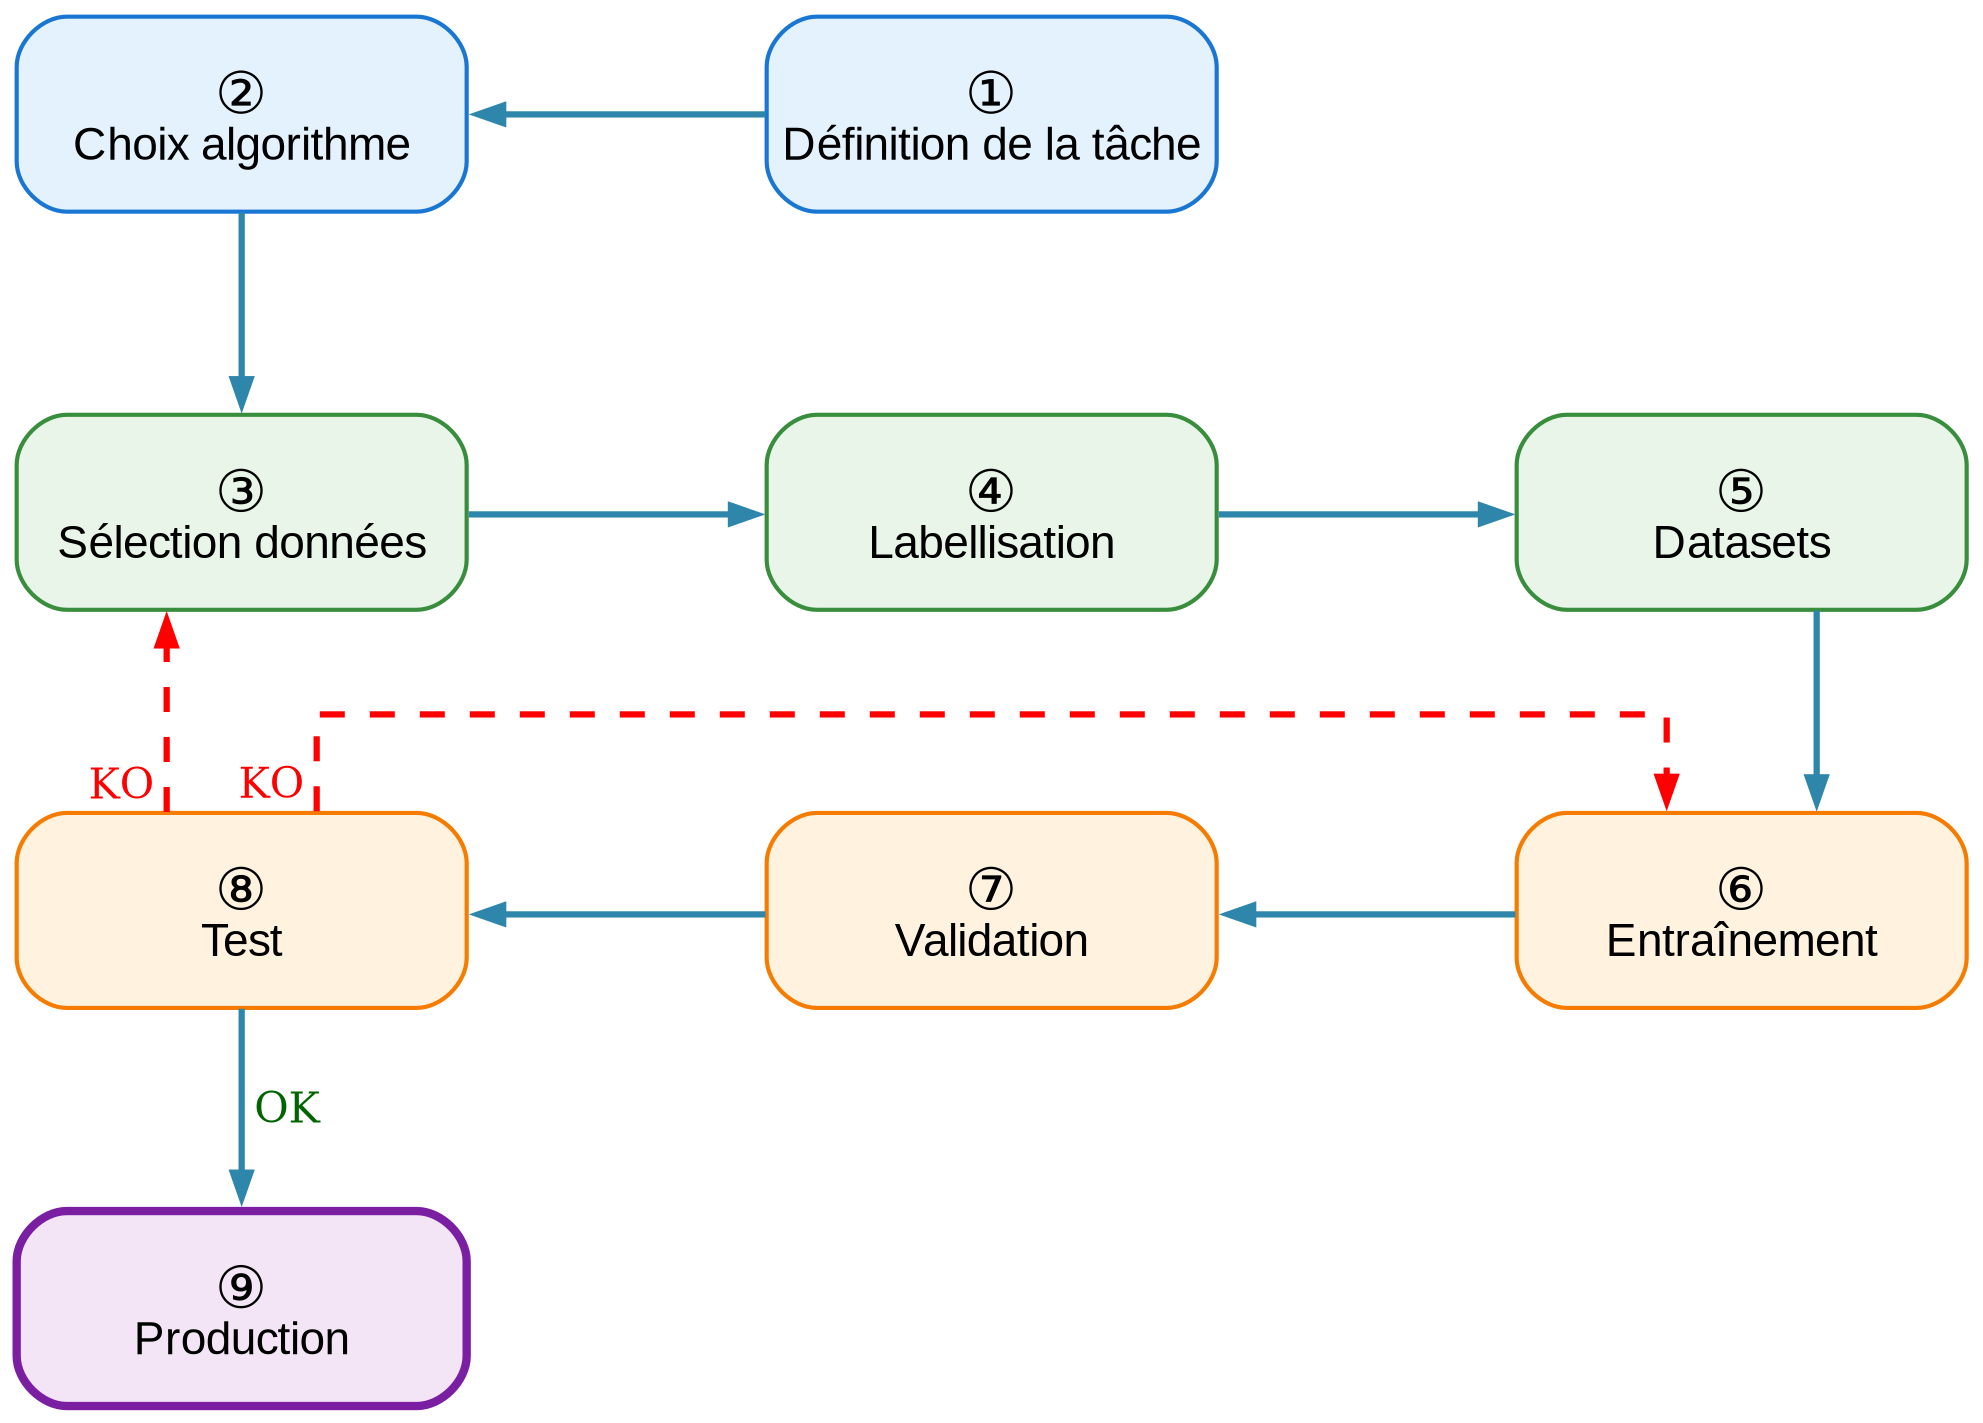
\includegraphics[width=1\linewidth]{03-tail/A1_fondamentaux_ML/A1_figures/A1_01_resume_machine_learning_supervise.png}
    \caption{Résumé du machine learning supervisé}
    \label{fig:A1_01_resume_machine_learning_supervise}
\end{figure}


\par{Un détail important pour la compréhension de la Figure~\ref{fig:A1_01_resume_machine_learning_supervise} est la différence entre modèle et algorithme :
\begin{itemize}
    \item Un modèle est une implémentation spécifique d'un algorithme, adaptée à un jeu de données ou un problème particulier.
    \item Un algorithme est un ensemble d'instructions ou une procédure utilisée pour entraîner un modèle.
\end{itemize}
}

\par{Une bonne manière de faire la différence est de voir l'algorithme comme la recette de cuisine et le modèle comme le gâteau. La recette (algorithme) fournit les instructions pour combiner les ingrédients, mais le gâteau (modèle) est le résultat physique de la mise en œuvre de la recette.}

\par{La Figure~\ref{fig:A1_01_resume_machine_learning_supervise} va servir de fil conducteur pour expliquer les principales phases :}

\begin{enumerate}
    \item Tâche : Le machine learning n'a pas de sens s'il n'y avait pas un problème à résoudre. Par exemple classer des images de chat et chien
    
    \item Choix algorithme : une fois la tâche déterminée, il faut choisir l'algorithme adéquat pour résoudre le problème. Par exemple choisir un algorithme de classification d'image
    
    \item Sélection des données adaptées à l'algorithme : la création du modèle nécessite des données appropriées à l'algorithme utilisé. Par exemple, des images de chats ou de chiens pour un algorithme de classification d'images.
    
    \item Ces données sont des exemples qui serviront à entraîner le modèle à effectuer des tâches spécifiques. Si les données ne sont pas étiquetées (également appelées annotées), il sera nécessaire de le faire. Dans le cas présent, il faudra rechercher des données déjà annotées de chats et de chiens, ou bien procéder à cette annotation soi-même. Ces données annotées constituent un ensemble de données (dataset ou jeu de données).
    
    \item Ces données doivent être divisée en plusieurs parties :
    \begin{enumerate}
        \item Données d'entraînement : elles serviront à l'entraînement du modèle et représentent environ 60\% du dataset.
        \item Données de validation : lors de l’entraînement ces données servent à valider que le modèle apprend correctement et qu'il ne mémorise pas les données d’entraînement. Les données de validation représentent environ 20\% du dataset
        \item Données de test : ces données ne sont pas utilisées lors de l'entraînement et servent à vérifier les performances finales du modèle sur des données qu'il n'a jamais vues auparavant. Les données de test représentent environ 20\% du dataset.
    \end{enumerate}
    
    \item Entraînement du modèle : on va appliquer l'algorithme sur les données \\ d’entraînement pour développer le modèle spécifique pour résoudre le problème de la première phase. Dans l'exemple, le modèle va apprendre les différentes caractéristiques d'un chien (museau, poil, etc.) et d'un chat.
    
    \item Validation des performances du modèle : le modèle est utilisé pour vérifier ses performances sur les données de validation. S'il arrive à bien classifier les chats ou les chiens, l’entraînement peut se terminer. Dans le cas où il n'arrive pas encore à bien les classifier, l’entraînement doit continuer.
    
    \item Test des performances du modèle : l'objectif de cette phase est d'évaluer les performances du modèle sur des données qu'il n'a jamais vues lors de l'entraînement. Les données utilisées sont les données de test. Si le modèle parvient à bien classifier les images de chats et de chiens (par exemple dans 85\% des cas), le modèle est considéré comme ``OK'' et peut passer en production. Cependant, si les performances ne sont pas satisfaisantes (cas ``KO''), il faut vérifier que les données sont adéquates, bien annotées et qu'il n'y a pas de problème de répartition entre les différentes classes. Une deuxième cause de mauvais résultats peut être le choix de variables (hyperparamètres) inadéquates pour l’entraînement.
    
    \item Mise en production : cette phase implique que le modèle fonctionne correctement et il peut maintenant réaliser la tâche pour laquelle il a été créé sur des données qu'il n'a jamais vues. Par exemple, classifier des images de chats et de chiens. La mise en production est complexe et souvent réalisée par des professionnels du DevOps qui ont d'excellentes connaissances des systèmes informatiques (``Ops'') ainsi que du développement informatique (``Dev''). Dans notre exemple, un site web pourrait accueillir l'interface dans laquelle l'utilisateur ou l'utilisatrice va soumettre une photo et le modèle va classifier l'image en chat ou en chien.
\end{enumerate}

\par{Le développement de modèles de machine learning supervisé est assez complexe et il se peut que cela ne fonctionne pas du premier coup (cas ``KO'' sur Figure~\ref{fig:A1_01_resume_machine_learning_supervise}). Les causes les plus habituelles sont les suivantes :}

\begin{itemize}
    \item Pas assez de données pour apprendre. Possible solution :
    \begin{itemize}
        \item Collecter plus de données
    \end{itemize}
    
    \item Équilibre des classes entre les données. Est-ce qu'une classe représente la majorité des données ? Est-ce que les chiens représentent par exemple plus de 80\% du dataset ? Si les données ne sont pas équilibrées, le modèle ne va pas bien apprendre les spécificités de chaque classe. Plusieurs solutions :
    \begin{itemize}
        \item Collecter plus de données de la ou les classe(s) moins représentée(s)
        \item S'il y a suffisamment de données, c'est possible d'enlever une partie des donnes jusqu'à ce que les classes soient équilibrées
    \end{itemize}
    
    \item Mauvais choix de modèle : c'est possible qu'un modèle soit trop complexe (réseau de neurones avec des milliards de paramètres) ou trop simple (régression linéaire). Possibles solutions :
    \begin{itemize}
        \item Vérifier que l'algorithme choisi est adapté à la tâche qu'il doit réaliser, il ne doit pas être trop simple ni trop complexe
        \item Si l'algorithme est complexe, c'est possible de le faire fonctionner avec plus de données mais ce n'est pas intelligent ni efficient d'un point de vue énergétique. Un gros modèle (beaucoup de paramètres) aura un entraînement plus long et va utiliser plus d'énergie lors de son utilisation
    \end{itemize}
\end{itemize}

\par{La réponse dans beaucoup de cas semble être d'acquérir plus de données. Cette démarche exige tout de même une certaine réflexion et dans certains cas ce n'est pas la meilleure :}

\begin{itemize}
    \item Coût de l'acquisition : l'acquisition de données supplémentaires peut être très coûteuse. Avoir plus de données va probablement impliquer la labellisation de celles-ci, ce qui peut engendrer des coûts non négligeables
    \item Rareté de la donnée : dans le domaine médical c'est difficile d'avoir plus de données sur des maladies rares par exemple
    \item Contraintes légales : des lois peuvent ne pas permettre l'accès à certaines données privées
    
    \item Qualité des données : la qualité de données collectées va avoir un impact sur le modèle, avoir des données de bonne qualité doit être une priorité par rapport à la quantité
\end{itemize}

% --------------------------------------------------------------------------------------------

\subsection{Applications}

\par{Le machine learning a des applications très variées et il est utilisé dans de nombreux domaines tels que :}

\begin{itemize}
    \item Vision par ordinateur (``computer vision'')
    \begin{itemize}
        \item Reconnaissance de caractères dans une image
        \item Générer automatiquement une description d'une image
        \item Conduite autonome d'un véhicule
        \item Aide au diagnostic de maladies dans le cadre de l'imagerie médicale
    \end{itemize}
    
    \item Traitement automatique du langage (``natural language processing'')
    \begin{itemize}
        \item Reconnaissance de voix automatique et transcription de ce qui est dit
        \item Traduction automatique de texte
        \item Classification de texte, par exemple classifier un courriel en ``spam'' ou un message dans un réseau social en ``language inapproprié''
        \item Modèles de language tel que GPT3.5 (ChatGPT) qui permettent de saisir des questions en texte et le modèle va générer une réponse dans le même format
    \end{itemize}
    
    \item Séries temporelles
    \begin{itemize}
        \item Planification prédictive du nombre de travailleurs nécessaires pour une entreprise
        \item Maintenance préventive de machines pour optimiser le nombre d'heures de fonctionnement
        \item Prédiction de météo et d'événements extrêmes tel que ouragans ou tremblements de terre
        \item Applications au domaine financier (ventes prévues d'une entreprise, aide à la décision dans les transactions boursières, etc.)
        \item Prédiction des embouteillages et aide à la gestion du trafic routier
        \item Aide à la gestion du réseau électrique en prédisant les pics de consommation
    \end{itemize}
\end{itemize}

% --------------------------------------------------------------------------------------------
\clearpage
\subsection{Neurones artificiels}

\par{Les réseaux de neurones sont très souvent utilisés en machine learning car ils permettent de résoudre des problèmes complexes et ils été une révolution dans le domaine.}

\par{Un réseau de neurones est un modèle mathématique inspiré de la structure et du fonctionnement du cerveau humain.}

\par{L'idée a été inspirée par le fonctionnement des neurones biologiques. C'est-à-dire que chaque neurone (voir Figure~\ref{fig:A1_02_neurone_humaine}) reçoit des signaux d'entrée de ses dendrites et produit des signaux de sortie le long de son axone. L'axone se ramifie ensuite et se connecte via des synapses aux dendrites d'autres neurones, formant ainsi un réseau neuronal.}

\begin{figure}[H]
    \centering
    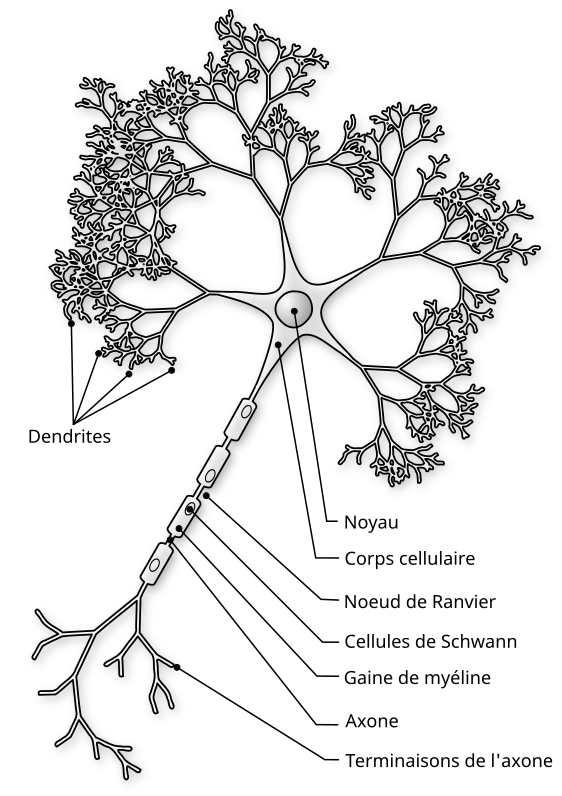
\includegraphics[width=0.85\linewidth]{03-tail//A1_fondamentaux_ML//A1_figures/A1_02_neurone_humaine.png}
    \caption{Neurone humaine \cite{noauthor_neurone_2025}}
    \label{fig:A1_02_neurone_humaine}
\end{figure}

\par{Le premier neurone artificiel \cite{mcculloch_logical_1943} a été créée en 1943 par Warren Sturgis McCulloch et Walter Pitts. La Figure~\ref{fig:A1_03_neurone_artificielle_mcculloch} permet de voir les similarités avec une neurone biologique. Le neurone de McCulloch-Pitts est une unité binaire avec un seuil d'activation qui reçoit une ou plusieurs entrées, effectue un calcul et produit une sortie.}

\begin{figure}
    \centering
    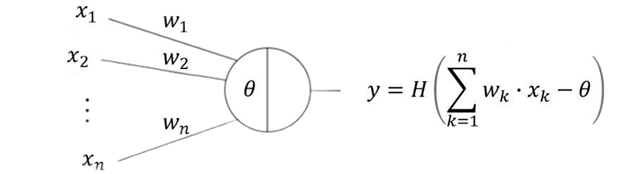
\includegraphics[width=1\linewidth]{03-tail//A1_fondamentaux_ML//A1_figures/A1_03_neurone_artificielle_mcculloch.png}
    \caption{Neurone artificielle proposée par McCulloch-Pitts \cite{zahn_cours_2024}}
    \label{fig:A1_03_neurone_artificielle_mcculloch}
\end{figure}

\par{Le neurone est constitué des parties suivantes :}
\begin{itemize}
    \item $x_1$, $x_2$, sont les entrées du neurone (signal), ce sont des signaux binaire qui prennent les valeurs de 0 ou 1
    \item $w_1$, $w_2$ sont les poids (``weights'') qui vont donner de l'importance au signal. Ils prennent les valeurs -1 (réduire le signal) ou +1 (augmenter le signal)
    \item $\theta$ est le seuil d'activation, c'est-à-dire la valeur minimum pour produire une sortie $y$
    \item $y$ est la valeur de sortie du neurone, c'est une valeur binaire
    \item $H$ est la formule d'activation
\end{itemize}

\par{L'activation utilise la fonction de Heaviside :}

\begin{equation}
    H(z) = 
    \begin{cases}
        0, & z < 0 \\
        1, & z \geq 0
    \end{cases}
    \label{eq:heaviside}
\end{equation}

\par{L'utilité de ce neurone est remarquable car il permet de créer des opérateurs logiques.}

\begin{equation}
    \begin{aligned}
        ET: \quad & y = H(x_1 + x_2 - 2) \\
        OU: \quad & y = H(x_1 + x_2 - 1) \\
        XOR: \quad & y = H(H(x_1 + x_2 - 1) + H(1 - x_1 - x_2))
    \end{aligned}
    \label{eq:operateurs_logiques}
\end{equation}

\par{Un exemple d'application de l'opérateur ``ET'' de l'Équation~\ref{eq:operateurs_logiques} permet de vérifier qu'il fonctionne correctement :}

\begin{equation}
    \begin{aligned}
        ET \quad \quad \quad & y = H(x_1 + x_2 - 2) \\
        \begin{cases}
            x_1 = 0 \\
            x_2 = 1
        \end{cases} \quad & y = H(0 + 1 - 2) \quad y = H(-1) = 0 \\
        \begin{cases}
            x_1 = 1 \\
            x_2 = 1
        \end{cases} \quad & y = H(1 + 1 - 2) \quad y = H(0) = 1
    \end{aligned}
    \label{eq:exemple_ET}
\end{equation}

\par{Ce modèle a certaines limitations :}
\begin{itemize}
    \item Ses poids ($w$) et seuil ($\theta$) sont fixes
    \item Sa sortie binaire ne permet pas de nuance, elle indique juste ``vrai'' (1) ou ``faux'' (0)
    \item Pas d'actualisations des poids selon les besoins
    \item Une seule couche ne permet pas de réaliser des calculs complexes
\end{itemize}

\par{En 1958, Frank Rosenblatt \cite{rosenblatt_perceptron_1958} publie un article ou il propose le perceptron, un nouveau type
de neurone artificiel.}
\begin{figure}[H]
    \centering
    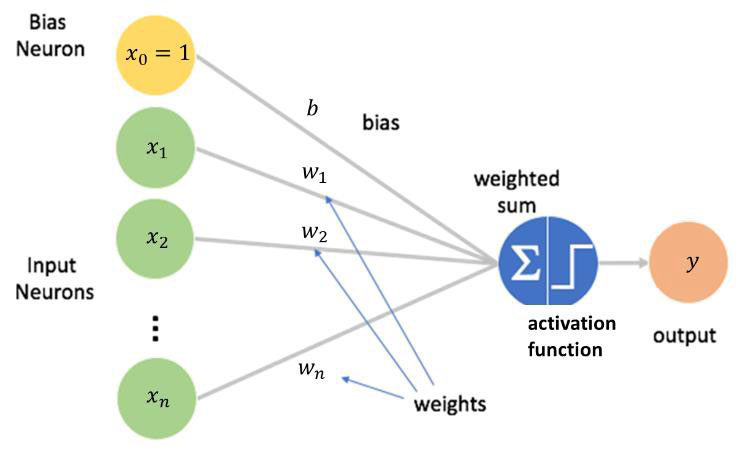
\includegraphics[width=1\linewidth]{03-tail//A1_fondamentaux_ML//A1_figures//A1_04_perceptron.png}
    \caption{Schéma du perceptron \cite{zahn_cours_2024}, neurone artificielle proposée par Frank Rosenblatt.}
    \label{fig:enter-label}
\end{figure}

\par{Celui-ci se distingue du neurone de McCulloch-Pitts car elle permet d'utiliser des nombres réels pour les entrées, poids et biais. L'équation \ref{eq:perceptron} \cite{rosenblatt_perceptron_1958} du perceptron est la suivante:}
\vspace{20pt}
\begin{equation}
    y = H\left(\sum_{k=1}^{n} w_k \cdot x_k + b\right) \quad \text{pour } x_k, w_k, b \in \mathbb{R}
    \label{eq:perceptron}
\end{equation}
\par{Dans l'équation \ref{eq:perceptron}, $H$ représente la fonction d'activation de Heaviside, $w_k$ les poids, $x_k$ les entrées, $b$ le biais, et $n$ le nombre d'entrées.}

\par{L'évolution la plus remarquable par rapport au neurone de McCulloch-Pitts, est que le perceptron peut « apprendre » des données et actualiser les poids et biais.}
\par{On dispose d'un ensemble de données étiquetées $\{(\mathbf{x}^{(i)}, y^{(i)})| i = 1, ... N\}$, où $\mathbf{x}^{(i)}$ sont des vecteurs $n$-dimensionnels. Pour la mise à jour des poids et du biais il faut suivre les étapes suivantes :}
\begin{enumerate}
    \item Initialiser le vecteur des poids $\mathbf{x}^{(i)}$ et le biais b avec des valeurs nulles (ou des valeurs aléatoires proches de 0)
    \item Itérer en mettant à jour le vecteur de poids $\mathbf{w}$ le biais b selon les règles suivantes :
    \begin{enumerate}
        \item Choisir un échantillon arbitraire : $(\mathbf{x}^{(i)}, y^{(i)})$
        \item Calculer la valeur prédite $\hat{y}^{(i)} = H(\mathbf{w} \cdot \mathbf{x}^{(i)} + b)$
        \item Utiliser la mise à jour des paramètres (équation \ref{eq:perceptron_maj1} et \ref{eq:perceptron_maj2} ci-dessous) :
        \vspace{20pt}
        \begin{align}
            \mathbf{w} &\leftarrow \mathbf{w} - \alpha \cdot (\hat{y}^{(i)} - y^{(i)}) \cdot \mathbf{x}^{(i)}
            \label{eq:perceptron_maj1}\\
            b &\leftarrow b - \alpha \cdot (\hat{y}^{(i)} - y^{(i)})
            \label{eq:perceptron_maj2}
        \end{align}
    \end{enumerate}
\end{enumerate}
\todo[inline]{Compléter}